\documentclass[12pt,a4paper]{article}

\usepackage[utf8]{inputenc}
\usepackage[T2A]{fontenc}
\usepackage[ukrainian]{babel}
\usepackage{geometry}
\usepackage{fancybox} % для рамки
\geometry{
    left=2cm,
    right=2cm,
    top=2cm,
    bottom=2cm
}

\usepackage[table]{xcolor}
\usepackage{amsmath}
\usepackage{graphicx}
\usepackage{subcaption} % обов'язково в преамбулі
\usepackage{multirow}  % Для об'єднання рядків
\usepackage{makecell}         % для багато­рядкових комірок
\usepackage{pdflscape}       % або можна використати lscape
\usepackage{booktabs}

\begin{document}

    \begin{titlepage}

        \thispagestyle{empty}
        \begin{center}
        \large
        Національний технічний університет України\\
        «Київський політехнічний інститут імені Ігоря Сікорського»\\[1em]
        Факультет інформатики та обчислювальної техніки\\
        Кафедра обчислювальної техніки
        \end{center}

        \vfill

        \begin{center}
        \textbf{\LARGE Комп'ютерна логіка. Частина 2}\\[2em]
        \textbf{\Large Лабораторна робота №6}\\
        «Дослідження операцій додавання та віднімання в двійково-кодованих системах числення» 
        \end{center}

        \vfill

        \begin{flushright}
        Виконав: студент 1 курсу ФІОТ, гр. ІО-41\\
        \textit{Давидчук А. М.}\\
        Залікова книжка № 4106\\[1em]
        Перевірив: \textit{Верба О.\,А.}
        \end{flushright}

        \vfill

        \begin{center}
        Київ -- 2025
        \end{center}

    \end{titlepage}

    \setlength{\parindent}{0pt}

    \textbf{\underline{Тема:}} «Дослідження операцій додавання та віднімання в двійково-кодованих системах числення».

    \vspace{1em}
    
    \textbf{\underline{Мета:}} Оволодіння способами подання десяткових чисел зі знаками. Дослідження операції додавання та віднімання чисел в системах числення з двійково-кодованим поданням цифр.

    \begin{center} \textbf{\large Виконання роботи} \end{center}

    \vspace{1em}

    \setlength{\parindent}{1.5em}

    Мій номер залікової книжки: 4106, що у двіковому вигляді є 0001 0000 0000 1010.
    Звідси $a_7 = 0, a_6 = 0, a_5 = 0, a_4 = 1, a_3 = 0, a_2 = 1, a_1 = 0$.
    Звідси визначу свій варіант з таблиці №1:

    \begin{table}[h!]
        \centering
        \renewcommand{\arraystretch}{1.2}
        \begin{tabular}{|c|c|c|c|c|c|}
        \hline
        $a_7a_6a_5$ & ДДК & $a_4a_3a_2$ & Логічні елементи & $a_3a_2a_1$ & \begin{tabular}{@{}c@{}}Операнди\\$X$\quad $Y$\end{tabular} \\
        \hline
        \cellcolor{yellow!45}000 & \cellcolor{yellow!45}8421+1 & 000 & 2І, 2АБО, НЕ & 000 & 3174 \quad -3442 \\
        001 & 8421+2 & 001 & 2І, 3АБО, НЕ & 001 & -3427 \quad 3626 \\
        010 & 8421+3 & 010 & 3І, 2АБО, НЕ & \cellcolor{yellow!45}010 & \cellcolor{yellow!45}-5473 \quad \cellcolor{yellow!45}3672 \\
        011 & 8421+4 & 011 & 3І, 3АБО, НЕ & 011 & 1234 \quad -7333 \\
        100 & 8421+5 & 100 & 2АБО-НЕ     & 100 & -5136 \quad 4437 \\
        101 & 2421   & \cellcolor{yellow!45}101 & \cellcolor{yellow!45}2І-НЕ        & 101 & -4512 \quad 1312 \\
        110 & 5421   & 110 & 3АБО-НЕ      & 110 & 5484 \quad -3445 \\
        111 & 7421   & 111 & 3І-НЕ        & 111 & 3342 \quad -3912 \\
        \hline
        \end{tabular}
        \caption{Таблиця логічних елементів та операндів}
    \end{table}

    Звідси кодування десяткових цифр в ДДК 8421+1:

    \begin{table}[h!]
        \centering
        \renewcommand{\arraystretch}{1.2}
        \begin{tabular}{|c|c|c|}
        \hline
        Десяткова цифра & Двійковий код (8421+1) \\
        \hline
        0 & 0001 \\
        1 & 0010 \\
        2 & 0011 \\
        3 & 0100 \\
        4 & 0101 \\
        5 & 0110 \\
        6 & 0111 \\
        7 & 1000 \\
        8 & 1001 \\
        9 & 1010 \\
        \hline
        \end{tabular}
        \caption{Кодування цифр від 0 до 9 у 8421+1 коді}
    \end{table}

    Оскільки дана ДДК має властивість адитивності, то перейдемо до створення
    таблиці істинності двійково-десятково суматора.

    \newpage

    \begin{table}[h!]
        \centering
        \renewcommand{\arraystretch}{1.2}
        \setlength{\tabcolsep}{4pt}
        \begin{tabular}{|c|c c c c c|c c c c c|c c c c|}
        \hline
        \rowcolor{gray!30}
        $\Sigma_{\text{д}}$ & $P_4'$ & $S_4'$ & $S_3'$ & $S_2'$ & $S_1'$ & $P_4$ & $S_4$ & $S_3$ & $S_2$ & $S_1$ & $S_4''$ & $S_3''$ & $S_2''$ & $S_1''$ \\
        \hline
        0  & 0  & 0 & 0 & 1 &  0 &   0 & 0 & 0 & 0 & 1   & 1 & 1 & 1 & 1 \\
        1  & 0  & 0 & 0 & 1 &  1 &   0 & 0 & 0 & 1 & 0   & 1 & 1 & 1 & 1 \\
        2  & 0  & 0 & 1 & 0 &  0 &   0 & 0 & 0 & 1 & 1   & 1 & 1 & 1 & 1 \\
        3  & 0  & 0 & 1 & 0 &  1 &   0 & 0 & 1 & 0 & 0   & 1 & 1 & 1 & 1 \\
        4  & 0  & 0 & 1 & 1 &  0 &   0 & 0 & 1 & 0 & 1   & 1 & 1 & 1 & 1 \\
        5  & 0  & 0 & 1 & 1 &  1 &   0 & 0 & 1 & 1 & 0   & 1 & 1 & 1 & 1 \\
        6  & 0  & 1 & 0 & 0 &  0 &   0 & 0 & 1 & 1 & 1   & 1 & 1 & 1 & 1 \\
        7  & 0  & 1 & 0 & 0 &  1 &   0 & 1 & 0 & 0 & 0   & 1 & 1 & 1 & 1 \\
        8  & 0  & 1 & 0 & 1 &  0 &   0 & 1 & 0 & 0 & 1   & 1 & 1 & 1 & 1 \\
        9  & 0  & 1 & 0 & 1 &  1 &   0 & 1 & 0 & 1 & 0   & 1 & 1 & 1 & 1 \\
        10 & 0  & 1 & 1 & 0 &  0 &   1 & 0 & 0 & 0 & 1   & 0 & 1 & 0 & 1 \\
        11 & 0  & 1 & 1 & 0 &  1 &   1 & 0 & 0 & 1 & 0   & 0 & 1 & 0 & 1 \\
        12 & 0  & 1 & 1 & 1 &  0 &   1 & 0 & 0 & 1 & 1   & 0 & 1 & 0 & 1 \\
        13 & 0  & 1 & 1 & 1 &  1 &   1 & 0 & 1 & 0 & 0   & 0 & 1 & 0 & 1 \\
        14 & 1  & 0 & 0 & 0 &  0 &   1 & 0 & 1 & 0 & 1   & 0 & 1 & 0 & 1 \\
        15 & 1  & 0 & 0 & 0 &  1 &   1 & 0 & 1 & 1 & 0   & 0 & 1 & 0 & 1 \\
        16 & 1  & 0 & 0 & 1 &  0 &   1 & 0 & 1 & 1 & 1   & 0 & 1 & 0 & 1 \\
        17 & 1  & 0 & 0 & 1 &  1 &   1 & 1 & 0 & 0 & 0   & 0 & 1 & 0 & 1 \\
        18 & 1  & 0 & 1 & 0 &  0 &   1 & 1 & 0 & 0 & 1   & 0 & 1 & 0 & 1 \\
        19 & 1  & 0 & 1 & 0 &  1 &   1 & 1 & 0 & 1 & 0   & 0 & 1 & 0 & 1 \\
        \hline
        \end{tabular}
        \caption{Таблиця істинності суматора для кодування 8421+1}
    \end{table}

    Після мінімізації функцій корекції отримуємо:
    $S_3'' = S_1'' = 1, P_4'' = \overline{S_4''} = \overline{S_2''} = S_4' S_3' \vee P_4' = \overline{\overline{S_4' S_3'} \land \overline{P_4'}}$

    \vspace{1em}

    \setlength{\parindent}{0pt}

    Комбінаційна схема формування корекції:

    \begin{figure}[ht]
        \centering
        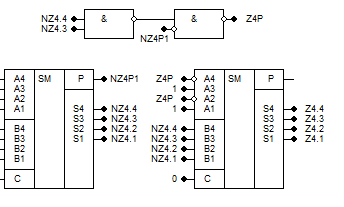
\includegraphics[width=0.5\textwidth]{1.png}
    \end{figure}

    \newpage

    Функціональна схема одного розряду двійково-десятково суматора:

    \begin{figure}[ht]
        \centering
        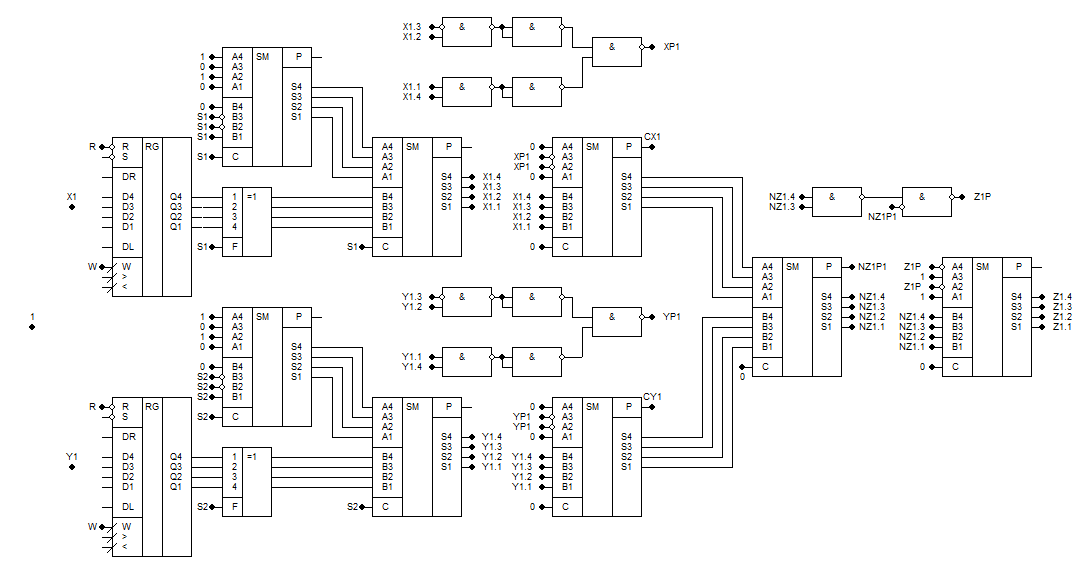
\includegraphics[width=1.00\textwidth]{2.png}
    \end{figure}

    Біти $S_1$ і $S_2$ визначають знаки чисел. Якщо число є від’ємним, його потрібно відняти від коду цифри 9. Проте, через те що ДДК 8421+1
    має надлишкове кодування, віднімати слід від коду числа 10 (тобто 9 + 1).

    \vspace{1em}

    Якщо у від'ємного числа перший розряд виявляється нульовим, результатом буде некоректний (недопустимий) код.
    Наприклад:

    \[
        \begin{array}{r@{\quad}r}
        (9_{10})    & 1010 \\
        (1_{10})    & +0001 \\
        (-0_{10})   & +1111 \\
                    & +0001 \\
                    & =1011 \\
        \end{array}
    \]

    Такий код корегується додавання 6 з переносом у старші розряди.

    \begin{center}
        \large Додавання X + Y
    \end{center}

    X = -5473 = 1.4527 = 1.0101 0110 0011 1000

    Y = 3672 = 0.3672 = 0.0100 0111 1000 0011

    Z = X + Y = 

    \vspace{1em}

    \makebox[0pt][l]{%
    \(
    \begin{array}{r}
    \phantom{+}1.4527 \\
    +0.3672 \\
    \hline
    = 1.8199 \\
    \end{array}
    \)
    }

    \vspace{1em}

    Звідси 1.8199 = -1801

    \newpage

    \begin{table}[ht]
    \begin{tabular}{|l|l|l|l|l|}
    \hline
    \multicolumn{1}{|l|}{
    \begin{tabular}{r@{\quad}r}
    0.   & 0101 \\
    +1.  & 0100 \\
    =1.  & 0 1001 \\
    \end{tabular}
    } &
    \begin{tabular}{r}
    0110 \\
    {+}0111 \\
    {=}0 1101 \\
    \end{tabular} &
    \begin{tabular}{r}
    0011 \\
    {+}1000 \\
    {=}0 1011 \\
    \end{tabular} &
    \begin{tabular}{r}
    1000 \\
    {+}0011 \\
    {=}0 1011 \\
    \end{tabular} & \\ \hline

    \multicolumn{1}{|l|}{
    \begin{tabular}{r@{\quad}r}
    +0.    & 0001 \\
    =1.  & 0 1010 \\
    +1.  & 1111 \\
    =1.  & 0 1001 \\
    \end{tabular}
    } & 
    \begin{tabular}{r}
    {+}0101 \\
    {=}1 0010 \\
    \end{tabular}& 
    \begin{tabular}{r}
    {+}1111 \\
    {=}0 1010 \\
    \end{tabular} &  
    \begin{tabular}{r}
    {+}1111 \\
    {=}0 1010 \\
    \end{tabular} & Корекція: -1, +5, -1, -1 \\ \hline
    \end{tabular}
    \end{table}

    Результат: 1.1001 0010 1010 1010 = 1.8199 = -1801; -5473 + 3672 = -1801; -1801 = -1801.

    \vspace{1em}

    Схема AFDK:

    \begin{figure}[ht]
        \centering
        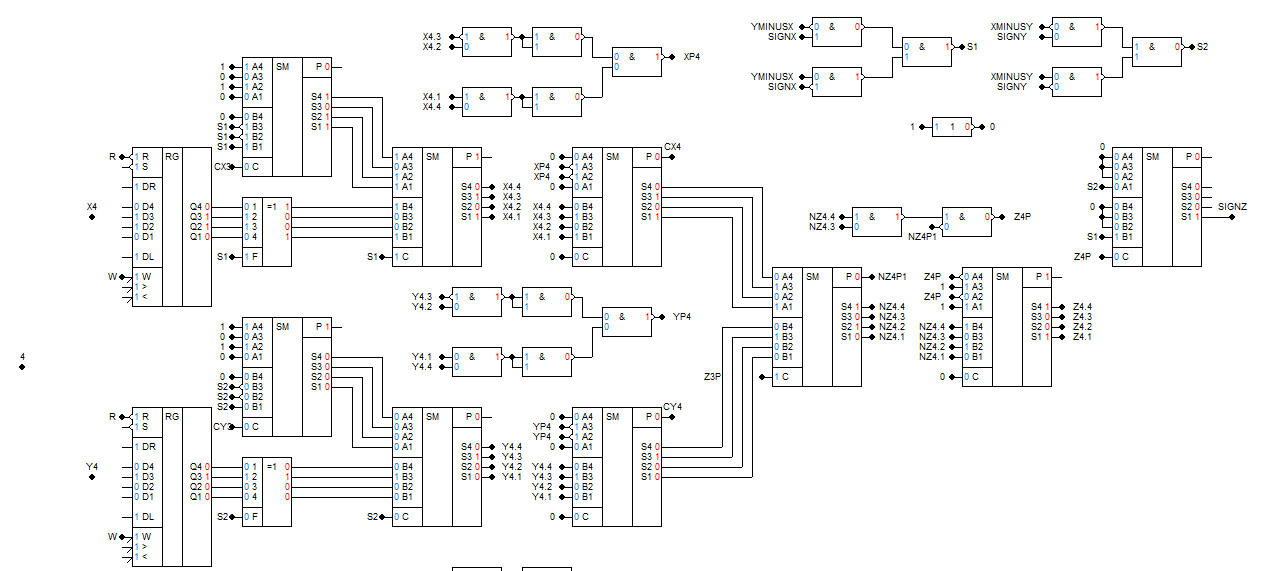
\includegraphics[width=0.89\textwidth]{1_1.png}
    \end{figure}

    \begin{figure}[ht]
        \centering
        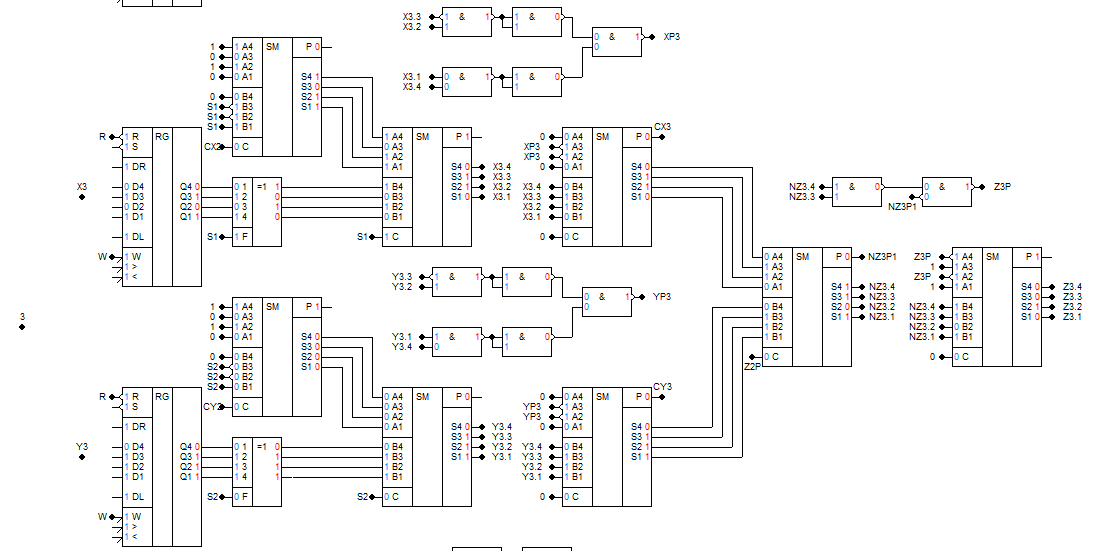
\includegraphics[width=0.89\textwidth]{1_2.png}
    \end{figure}

    \newpage

    \begin{figure}[ht]
        \centering
        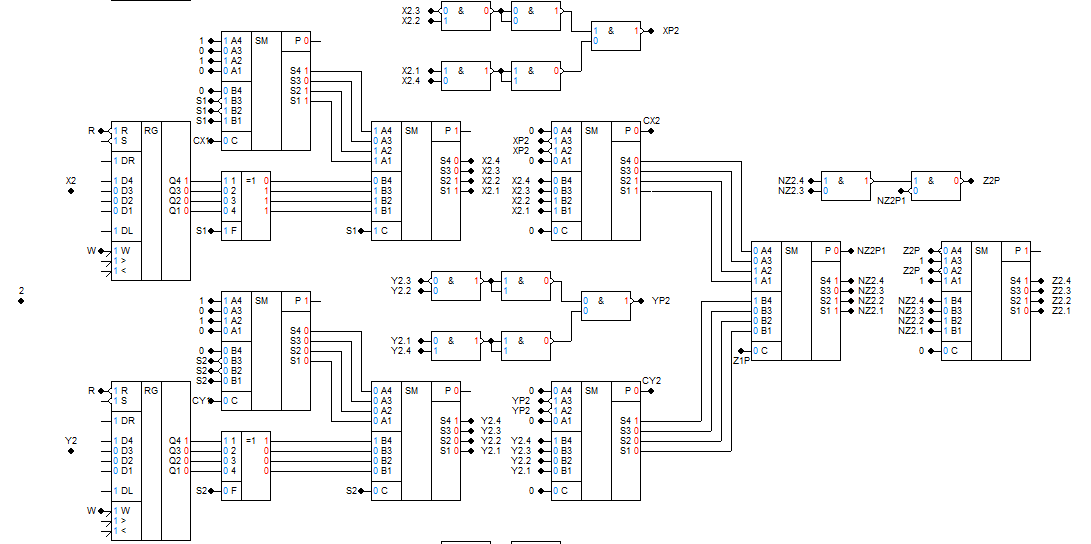
\includegraphics[width=0.89\textwidth]{1_3.png}
    \end{figure}

    \begin{figure}[ht]
        \centering
        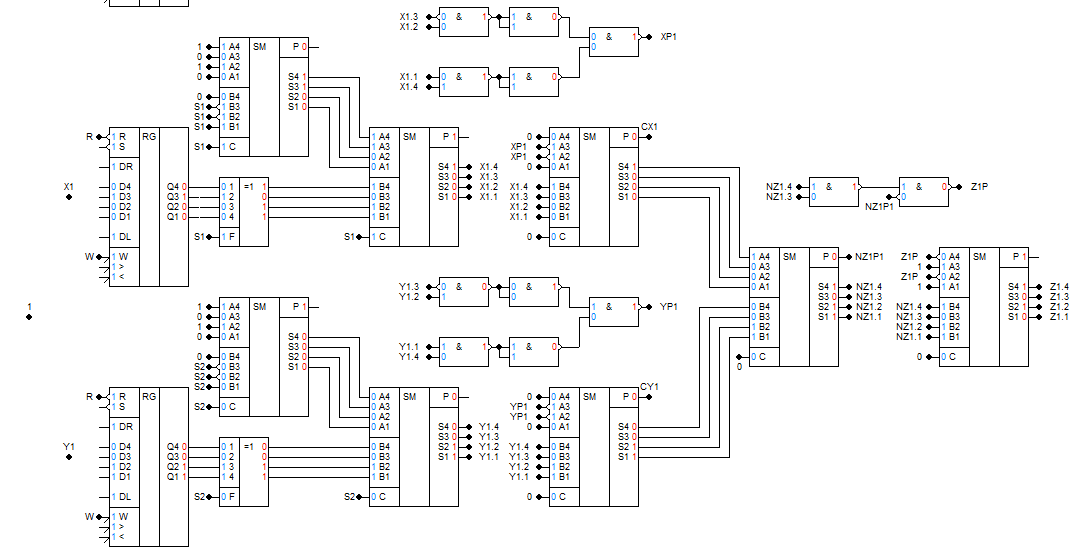
\includegraphics[width=0.89\textwidth]{1_4.png}
    \end{figure}

    \begin{center}
        \large Віднімання Z = X + (-Y)
    \end{center}

    X = -5473 = 1.4527 = 1.0101 0110 0011 1000

    -Y = -3672 = 1.9328 = 1.0111 0100 0011 1001

    Z = X + (-Y):

    \vspace{1em}

    \makebox[0pt][l]{%
    \(
    \begin{array}{r}
    \phantom{+}1.4527 \\
    +1.6328 \\
    \hline
    = 1.0855 \\
    \end{array}
    \)
    }

    \vspace{1em}

    Звідси 1.0855 = -9145

    \newpage

    \begin{table}[ht]
    \begin{tabular}{|l|l|l|l|l|}
    \hline
    \multicolumn{1}{|l|}{
    \begin{tabular}{r@{\quad}r}
    1.   & 0101 \\
    +1.  & 0111 \\
    =0.  & 0 1100 \\
    \end{tabular}
    } &
    \begin{tabular}{r}
    0110 \\
    {+}0100 \\
    {=}0 1010 \\
    \end{tabular} &
    \begin{tabular}{r}
    0011 \\
    {+}0011 \\
    {=}0 0111 \\
    \end{tabular} &
    \begin{tabular}{r}
    1000 \\
    {+}1001 \\
    {=}1 0001 \\
    \end{tabular} & \\ \hline

    \multicolumn{1}{|l|}{
    \begin{tabular}{r@{\quad}r}
    +0.    & 0101 \\
    =1.  & 1 0001 \\
    \end{tabular}
    } & 
    \begin{tabular}{r}
    {+}1111 \\
    {=}1 1001 \\
    \end{tabular}& 
    \begin{tabular}{r}
    {+}1111 \\
    {=}0 0110 \\
    \end{tabular} &  
    \begin{tabular}{r}
    {+}0101 \\
    {=}0 0110 \\
    \end{tabular} & Корекція: +5, -1, -1, +5 \\ \hline
    \end{tabular}
    \end{table}

    Результат: 1.0001 1001 0110 0110 = 1.0855 = -9145; -5473 + (-3672) = -9145; -9145 = -9145.

    \vspace{1em}

    Схема AFDK:

    \begin{figure}[ht]
        \centering
        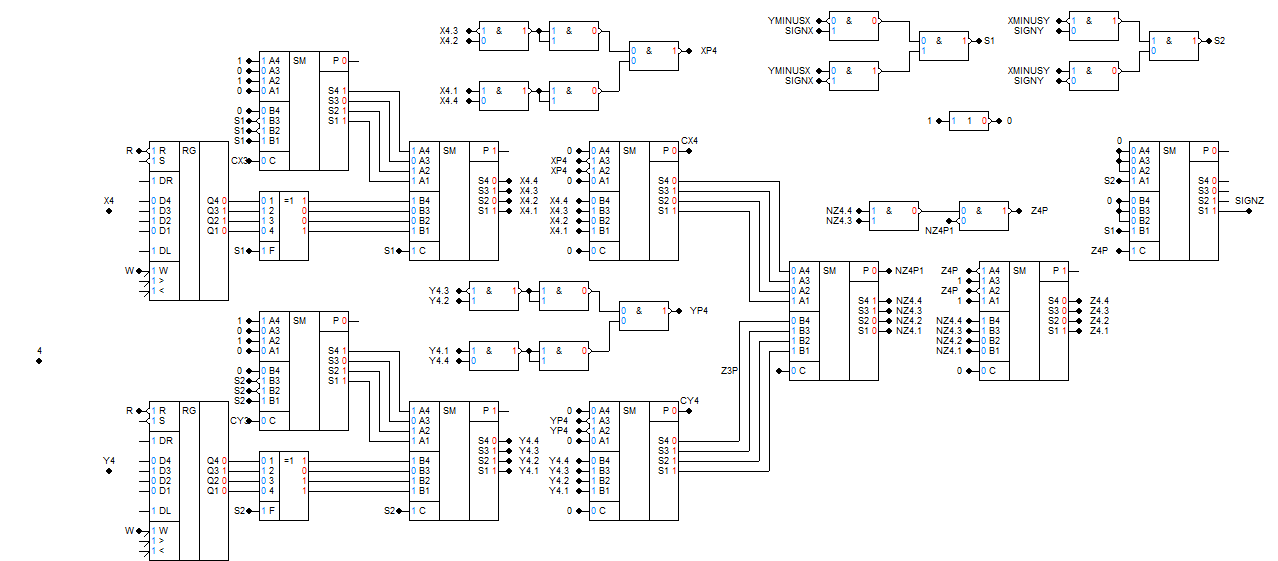
\includegraphics[width=0.89\textwidth]{2_1.png}
    \end{figure}

    \begin{figure}[ht]
        \centering
        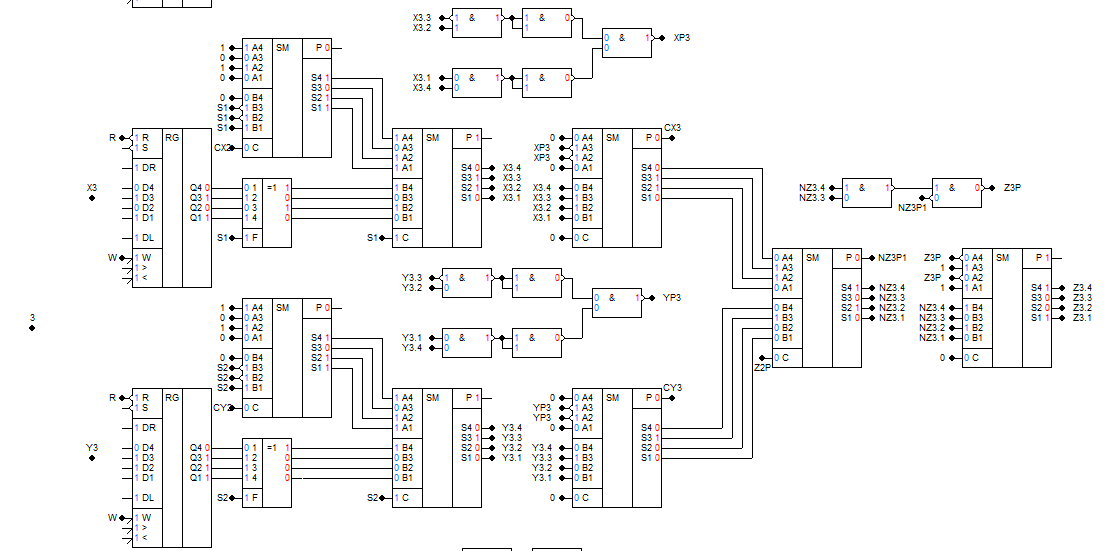
\includegraphics[width=0.89\textwidth]{2_2.png}
    \end{figure}

    \newpage

    \begin{figure}[ht]
        \centering
        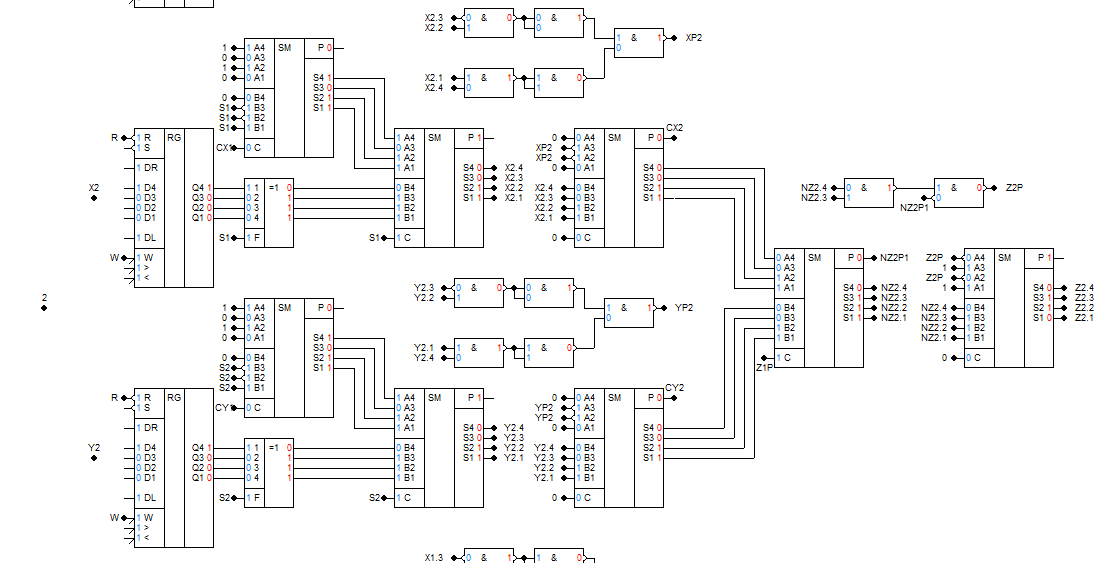
\includegraphics[width=0.89\textwidth]{2_3.png}
    \end{figure}

    \begin{figure}[ht]
        \centering
        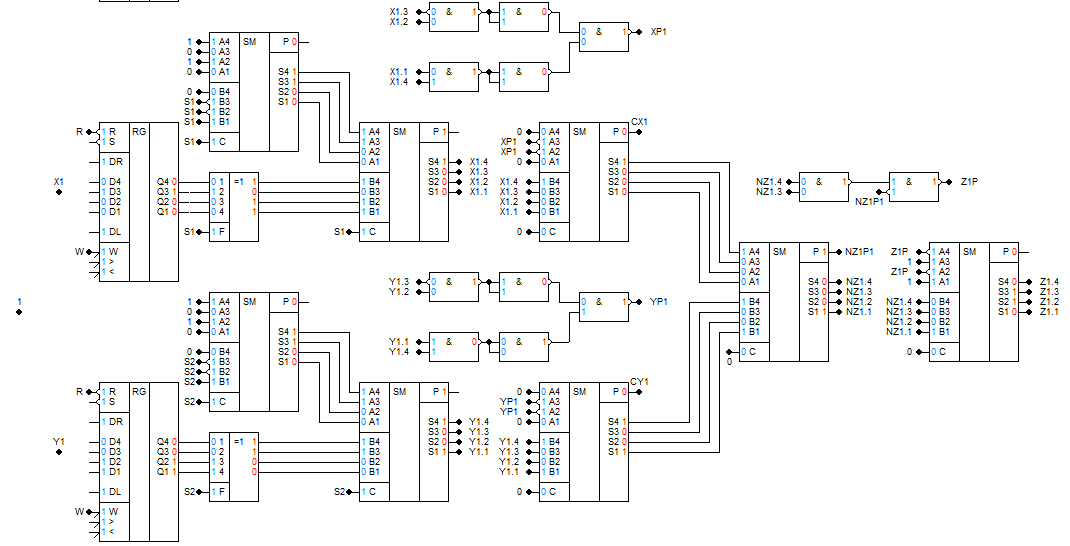
\includegraphics[width=0.89\textwidth]{2_4.png}
    \end{figure}

    \begin{center}
        \large Віднімання Z = Y + (-X)
    \end{center}

    -X = 5473 = 0.5473 = 0.0110 0101 1000 0100

    Y = 3672 = 0.3672 = 0.0100 0111 1000 0011

    \vspace{1em}

    Z = Y + (-X):

    \vspace{1em}

    \makebox[0pt][l]{%
    \(
    \begin{array}{r}
    \phantom{+}0.5473 \\
    +0.3672 \\
    \hline
    = 0.9145 \\
    \end{array}
    \)
    }

    \vspace{1em}

    Звідси 0.9145 = 9145

    \newpage

    \begin{table}[ht]
    \begin{tabular}{|l|l|l|l|l|}
    \hline
    \multicolumn{1}{|l|}{
    \begin{tabular}{r@{\quad}r}
    0.   & 0110 \\
    +0.  & 0100 \\
    =0.  & 0 1010 \\
    \end{tabular}
    } &
    \begin{tabular}{r}
    0101 \\
    {+}0111 \\
    {=}0 1101 \\
    \end{tabular} &
    \begin{tabular}{r}
    1000 \\
    {+}1000 \\
    {=}1 0000 \\
    \end{tabular} &
    \begin{tabular}{r}
    0100 \\
    {+}0011 \\
    {=}1 0111 \\
    \end{tabular} & \\ \hline

    \multicolumn{1}{|l|}{
    \begin{tabular}{r@{\quad}r}
    +0.    & 0001 \\
    =0.  & 0 1011 \\
    +0.  & 1111 \\
    =0.  & 0 1010 \\
    \end{tabular}
    } & 
    \begin{tabular}{r}
    {+}0101 \\
    {=}1 1001 \\
    \end{tabular}& 
    \begin{tabular}{r}
    {+}0101 \\
    {=}0 0110 \\
    \end{tabular} &  
    \begin{tabular}{r}
    {+}1111 \\
    {=}0 0110 \\
    \end{tabular} & Корекція: -1, +5, +5, -1 \\ \hline
    \end{tabular}
    \end{table}

    Результат: 0.1010 0010 0101 0110 = 0.9145 = 9145; 5473 + 3672 = 9145; 9145 = 9145.

    \vspace{1em}

    Схема AFDK:

    \begin{figure}[ht]
        \centering
        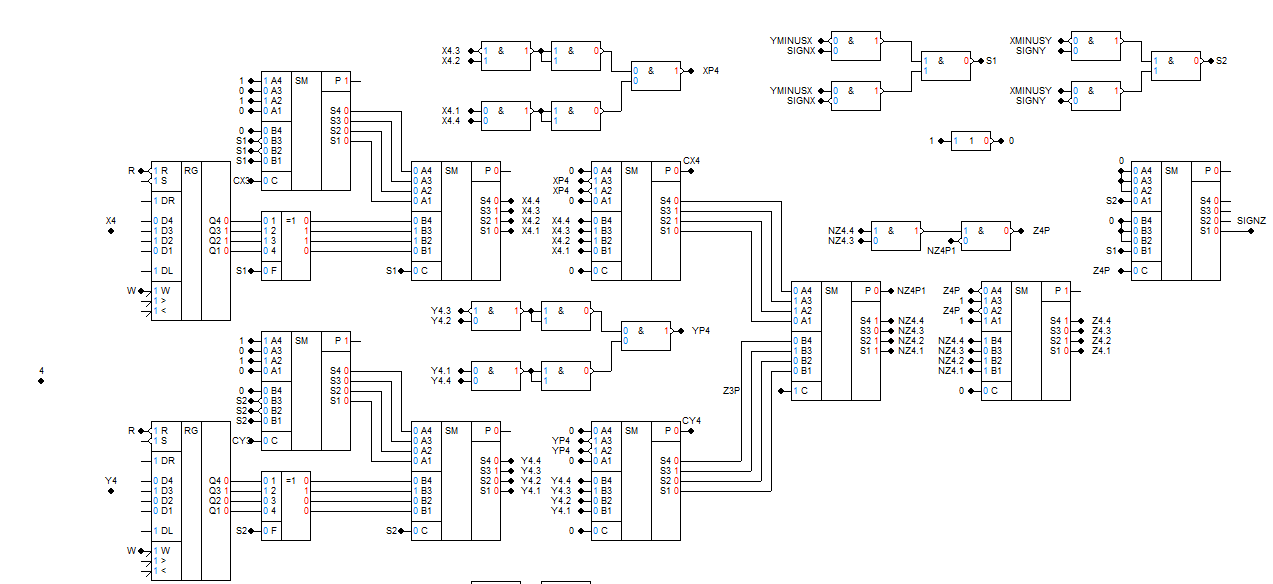
\includegraphics[width=0.89\textwidth]{3_1.png}
    \end{figure}

    \begin{figure}[ht]
        \centering
        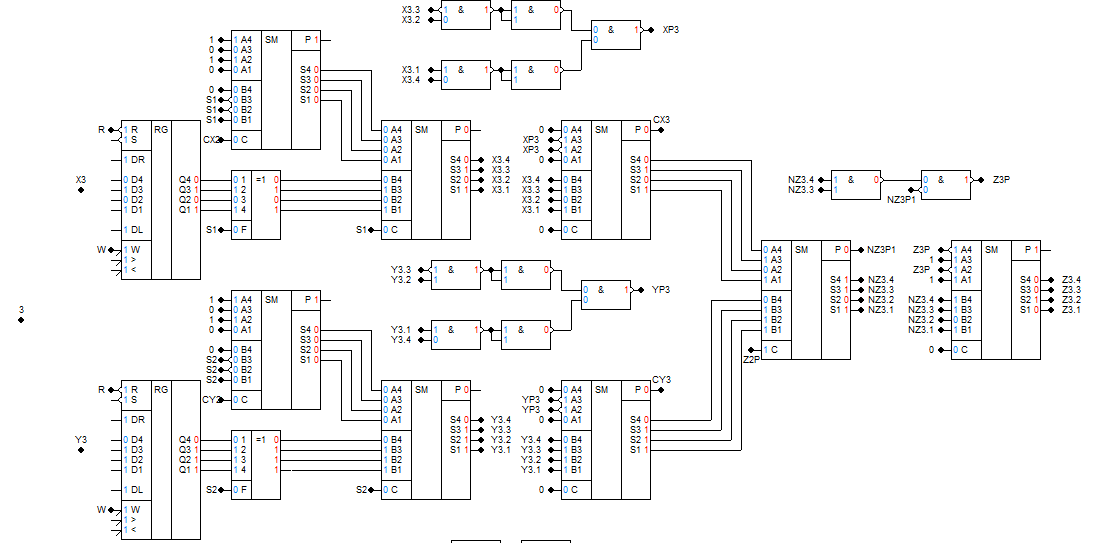
\includegraphics[width=0.89\textwidth]{3_2.png}
    \end{figure}

    \newpage

    \begin{figure}[ht]
        \centering
        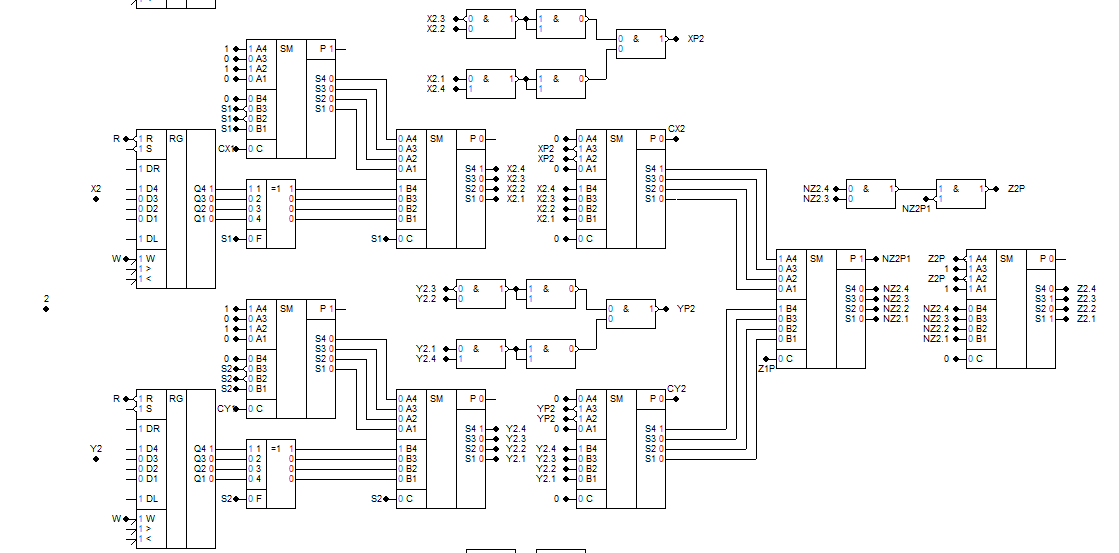
\includegraphics[width=0.89\textwidth]{3_3.png}
    \end{figure}

    \begin{figure}[ht]
        \centering
        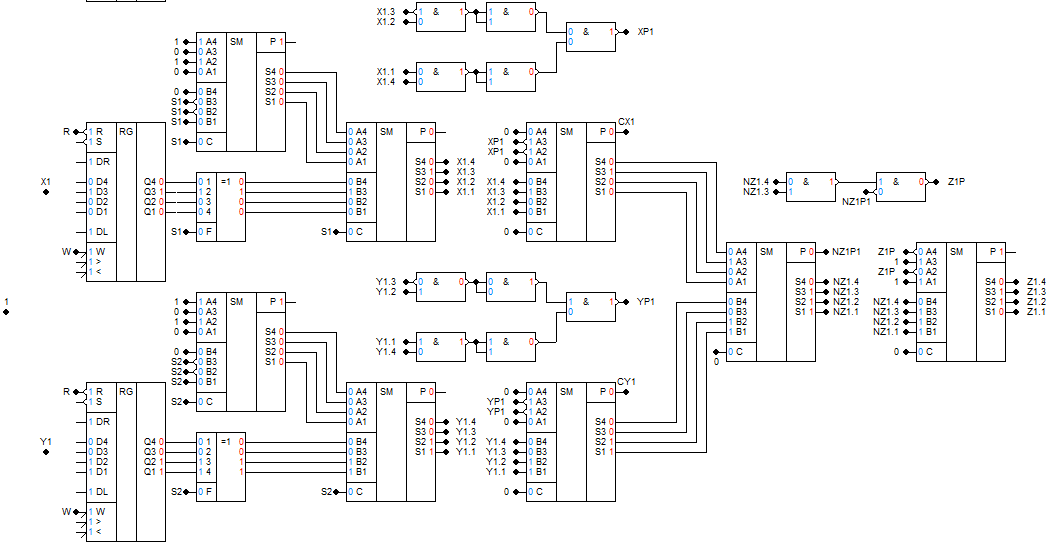
\includegraphics[width=0.89\textwidth]{3_4.png}
    \end{figure}

    \textbf{\underline{Висновок:}}
    У процесі виконання лабораторної роботи я ознайомився з основами двійково-десяткового кодування, зокрема варіантом ДДК 8421+1. Було розглянуто його структуру, принципи подання чисел та виконання арифметичних операцій у межах цієї системи. Особливу увагу приділено механізму переносу та алгоритмам корекції результатів, що є необхідними для забезпечення правильності обчислень у ДДК.
У практичній частині я реалізував операції додавання та віднімання в коді 8421+1, а також побудував логічні схеми суматорів. Це дозволило глибше зрозуміти принципи роботи цифрових обчислювальних пристроїв і процес реалізації обчислень на апаратному рівні.

    \newpage

    \begin{center} \textbf{\large Контрольні питання} \end{center}

    \vspace{1em}

    \begin{enumerate}
    \item \textbf{В якій формі  у ЕОМ подаються десяткові числа?} \\
    У ЕОМ десяткові числа можуть подаватися у формі чисел з плаваючою комою або у формі цілих чисел. У формі чисел з плаваючою комою десяткове число представлене у вигляді десяткової дробу, де кома може знаходитися в будь-якому місці числа, вказуючи позицію між цифрами. У формі цілих чисел десяткове число подається без дробової частини, як ціле число.

    \vspace{1em}

    \item \textbf{Як визначити кількість розрядів двійкового і двійково-десяткового числа з однаковим кількісним еквівалентом?} \\
    Для представлення однієї цифри необхідно мати не менше ніж $m = \left\lceil \log_2(k - 1) \right\rceil$
    двійкових розрядів ($\left\lceil ... \right\rceil$ --- функція округлення числа до найбільшого цілого).
    Наприклад, для десяткової системи числення цифри кодуються не менш ніж чотирма двійковими розрядами (тетрадами), хоча двійково-десяткові коди (ДДК) можуть мати і більше розрядів, якщо це дає переваги при виконанні певних операцій.

    \vspace{1em}

    \item \textbf{Поясніть, коли при додаванні чисел необхідна корекція результату.} \\
    В коді 8421 корекція в десяткових розрядах виконується, якщо після підсумування тетрад виникає перенос в старшу тетраду або результат в тетраді стає більше 9.

    \vspace{1em}

    \item \textbf{Як визначити необхідну корекцію при додаванні двійково-десяткових чисел?} \\
    Одиниця, що залишає тетраду, повинна забрати з неї $k=10$ одиниць, а фактично забирає 16, тобто подвійну вагу старшого двійкового розряду тетради
    (для коду 8421 ця вага дорівнює 8). Тому для компенсації до тетради додається число +6 ($0110_2$) з розповсюдженням переносу в старшу тетраду.

    \vspace{1em}

    \item \textbf{Наведіть склад апаратури для побудови двійково-десяткового суматора.} \\
    Двійково-десяткові суматори в кожному десятковому розряді повинні реалізувати п'ять
    перемикальних функцій.
    Чотири з них відповідають двійково-кодованій десятковій сумі $S = s_4s_3s_2s_1$
    і одна - переносу в старший десятковий розряд $P_4$.
    Ці функції залежать від десяткових цифр доданків $X = x_4x_3x_2x_1$ і $Y = y_4y_3y_2y_1$,
    а також переносу з молодшої тетради $P_0$, тобто від 9 аргументів. Нормальні форми функцій дуже громіздкі і погано мінімізуються. Тому підсумування ДДК доцільно виконувати відповідно до схеми.
    На першому етапі на двійковому суматорі підсумовують ДДК десяткових цифр за правилами двійковій арифметики. Потім на другому етапі за допомогою ще одного суматора роблять корекцію отриманого результату шляхом додавання або віднімання деякої константи, що визначається комбінаційною схемою КС, а також виділяють десятковий перенос в старшу тетраду.

    \vspace{1em}

    \item \textbf{Яким вимогам повинні задовольняти ДДК, що використовуються у суматорі?} \\
    ДДК повинен мати властивості адитивності. Такою властивістю володіють ДДК 8421 і $8421+\Delta$, де --- $\Delta$ ціле число, що назване надлишком. Якщо використовується ДДК, що не володіє властивостями адитивності, то цифри доданків слід перед підсумовуванням перетворити в адитивний ДДК.

    \vspace{1em}

    \item \textbf{У чому сутність властивості адитивності ДДК і до чого може призвести її відсутність?} \\
    Адитивність — можливість виконувати додавання на рівні кодів. Відсутність цієї властивості призводить до некоректних результатів або складніших схем корекції.

    \vspace{1em}

    \item \textbf{У чому сутність властивості зваженості ДДК і до чого може призвести її відсутність?} \\
    Зваженість означає відповідність кожного біта певній вазі. Наприклад, у коді 8421 — ваги $8,4,2,1$. Втрата зваженості унеможливлює пряме перетворення між системами числення.

    \vspace{1em}

    \item \textbf{Наведіть приклади ДДК, що володіють і не володіють властивістю адитивності.} \\
    Код 2421 --- ДДК зі штучним порядком ваг. Він має всі властивості, крім властивості адитивності, оскільки старший розряд тетради має штучну вагу 2. Цей код є само доповняльним і використовується при виконанні арифметичних операцій над десятковими числами у зворотному або доповняльному коді.

    \vspace{1em}

    \item \textbf{Наведіть приклади ДДК, що володіють і не володіють властивістю зваженості.} \\
    Код з «надлишком» не має властивості зваженості, оскільки отримується в результаті додавання двійкового коду цифри 3 (0011) до кожної цифри коду прямого заміщення ($N+3$). Код є не зручним для перетворення з однієї СЧ в іншу але він зручний для виконання арифметичних операцій над десятковими числами. 
    При цьому легко отримати перенос, оскільки сума двох доданків кожне з яких беруть з надлишком 3 отримується з надлишком 6, що виключає зайві кодові комбінації (для отримання правильного коду суми від результату віднімається 6). 
    Серед незважених ДДК можна відмітити коди спеціального призначення, в яких перехід до суміжного числа супроводжується змінами тільки в одному розряді (коди з обмінною одиницею).

    \vspace{1em}

    \item \textbf{Наведіть приклад додавання 4-розрядних двійково-десяткових чисел із знаками в заданому ДДК.} \\
    \noindent
    \doublebox{%
    \begin{tabular}{@{}r@{ }c@{ }l@{}}
    3829\textsubscript{2--10} & = & 0.0011 1000 0010 1001 \\
    +1658\textsubscript{2--10} & = & 0.0001 0110 0101 1000 \\
                            & = & 0.0100 1110 1000 0001 \\
    Корекція:                 & + & 0.0000 0110 0000 0110 \\
    5487\textsubscript{2--10} & = & 0.0101 0100 1000 0111 \\
    \end{tabular}
    }

\end{enumerate}

\end{document}